\documentclass[9pt]{IEEEtran}

\usepackage[english]{babel}
\usepackage{graphicx}
\usepackage{epstopdf}
\usepackage{fancyhdr}
\usepackage{amsmath}
\usepackage{amsthm}
\usepackage{amssymb}
\usepackage{url}
\usepackage{array}
\usepackage{textcomp}
\usepackage{listings}
\usepackage{hyperref}
\usepackage{xcolor}
\usepackage{colortbl}
\usepackage{float}
\usepackage{gensymb}
\usepackage{longtable}
\usepackage{supertabular}
\usepackage{multicol}

\usepackage[utf8x]{inputenc}

\usepackage[T1]{fontenc}
\usepackage{lmodern}{}
\input{glyphtounicode}
\pdfgentounicode=1

\graphicspath{{./figures/}}
\DeclareGraphicsExtensions{.pdf,.png,.jpg,.eps}

% correct bad hyphenation here
\hyphenation{op-tical net-works semi-conduc-tor trig-gs}

% ============================================================================================

\title{\vspace{0ex}
Bayesian Inference}

\author{Marko Medved\vspace{-4.0ex}}

% ============================================================================================

\begin{document}

\maketitle

\section{Implementation of the Poisson GLM with Bayesian inference using MCMC}

\subsection{Implementation details}

For this part of the assignment, we implemented a Poisson
 Generalized Linear Model (GLM) using Bayesian inference. As
  a preprocessing step, we standardized all predictor variables.
   For the prior distribution of 
  the regression coefficients ($\beta$), we used a normal distribution
   with zero mean and a large variance ($\alpha = 10$). This
    choice reflects a weakly informative prior—wide enough to avoid 
    imposing strong constraints on the coefficients,
     allowing the data to primarily inform the posterior.

To perform inference, we used the Markov Chain Monte Carlo (MCMC)
 method to sample from the posterior distribution. To assess 
 convergence reliably, we ran 4 independent chains. Each chain 
 generated 1000 posterior samples following a burn-in phase of 1000
  iterations.

\subsection{Relationship between the explanatory and GoalsScored variables}
To describe the relationship between features and the target variable, 
we plot the posterior densities of the regression coefficients in
 Figure~\ref{fig:densities}. The Score Rate of the home team stands 
 out as the most important feature, showing a clear positive effect
  on the expected number of goals.
   In contrast, the home team’s foul ratio (somewhat unexpectedly) 
   and concede rate (as expected) have the strongest negative 
   effects, reducing the predicted goal count. Other coefficients are
    close to zero, indicating little effect since their multiplicative 
    impact on the mean is near one after applying the link function. 
    The intercept was excluded from this visualization for clarity but 
    shows a similar distribution centered around one.

The similar widths of the coefficient distributions suggest comparable 
uncertainty across all features. This is also confirmed when looking at the 
standard deviations which are roughly the same for all coefficients. 


\begin{figure}[h]
\centering
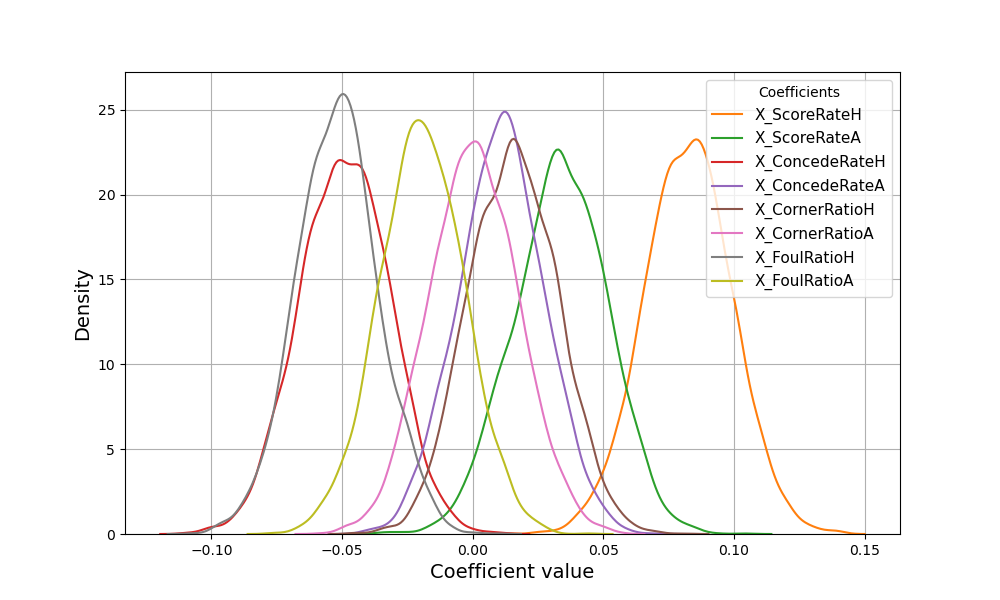
\includegraphics[width=1\columnwidth]{figures/densities.png}
\caption{Densities of coefficients for the features with the exclusion of the 
intercept density}
\label{fig:densities}
\end{figure}



\subsection{MCMC diagnostics}
We use standard MCMC diagnostics to assess convergence.
 Figure~\ref{fig:trace} shows the trace plots of all 
 regression coefficients across the 4 chains. The samples 
 for each parameter appear stable and well-mixed, with no 
 visible trends, and the chains overlap closely—indicating good convergence.


\begin{figure}[h]
\centering
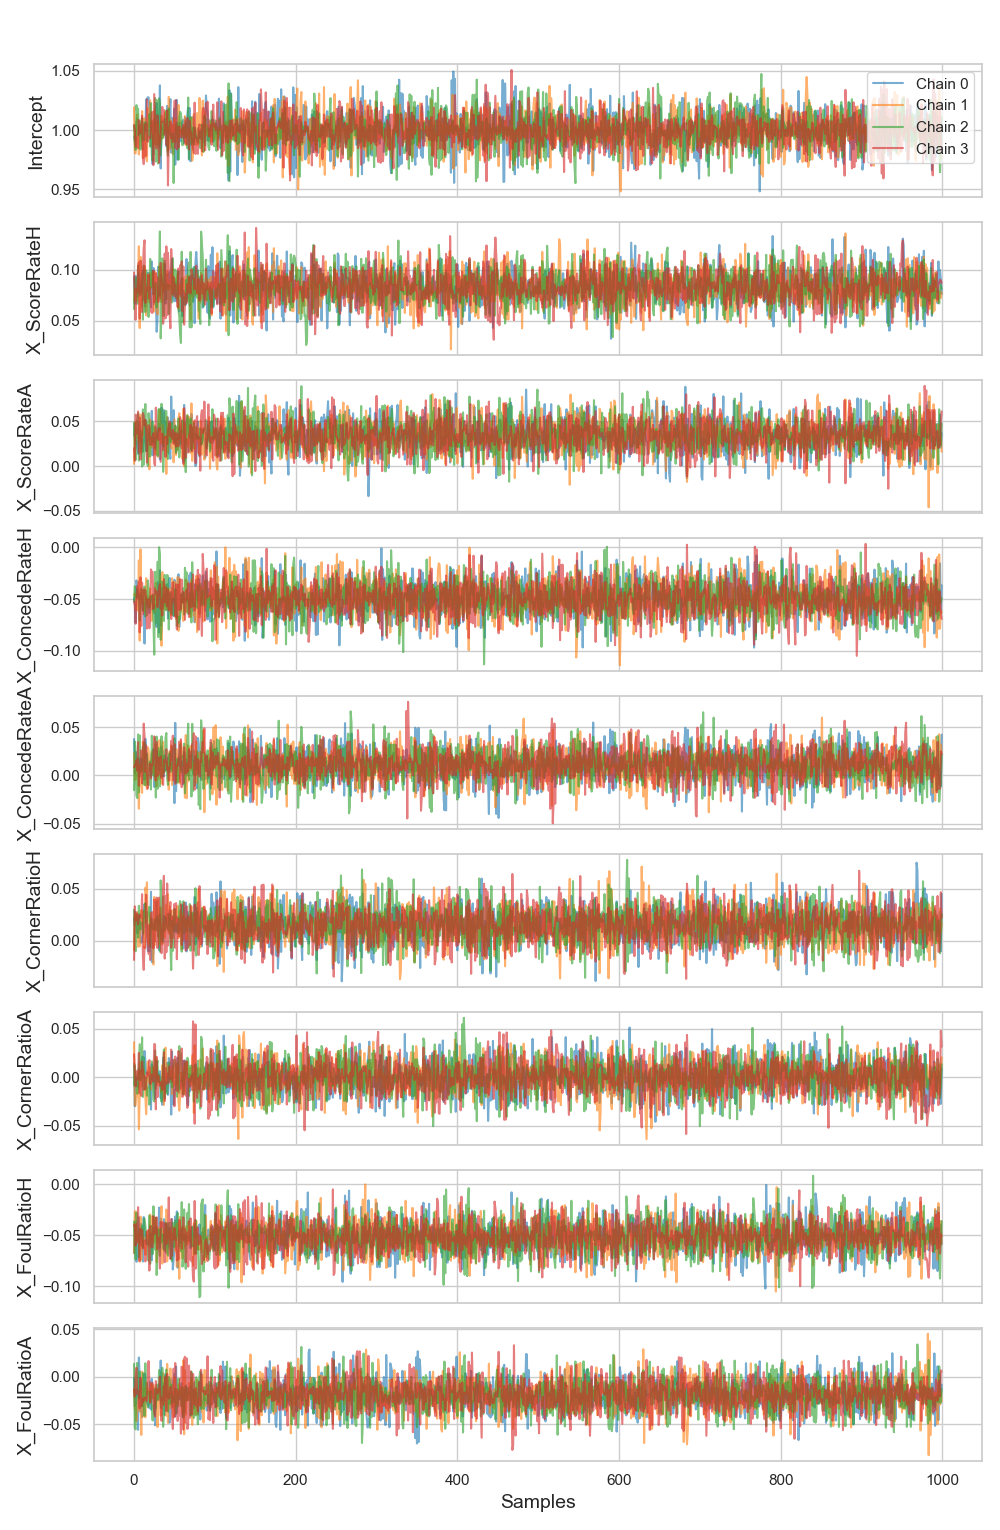
\includegraphics[width=1\columnwidth]{figures/trace.png}
\caption{Trace plots for each of the regression coefficients for one of the chains}
\label{fig:trace}
\end{figure}

In Figure~\ref{fig:autocorr}, we present the autocorrelation 
plots for all the regression coefficients 
(only for one chain to save space). The autocorrelations
 across  coefficients and lags are close to zero, with some of them even being
 negative, indicating that the samples are really nicely uncorrelated.

\begin{figure}[h]
\centering
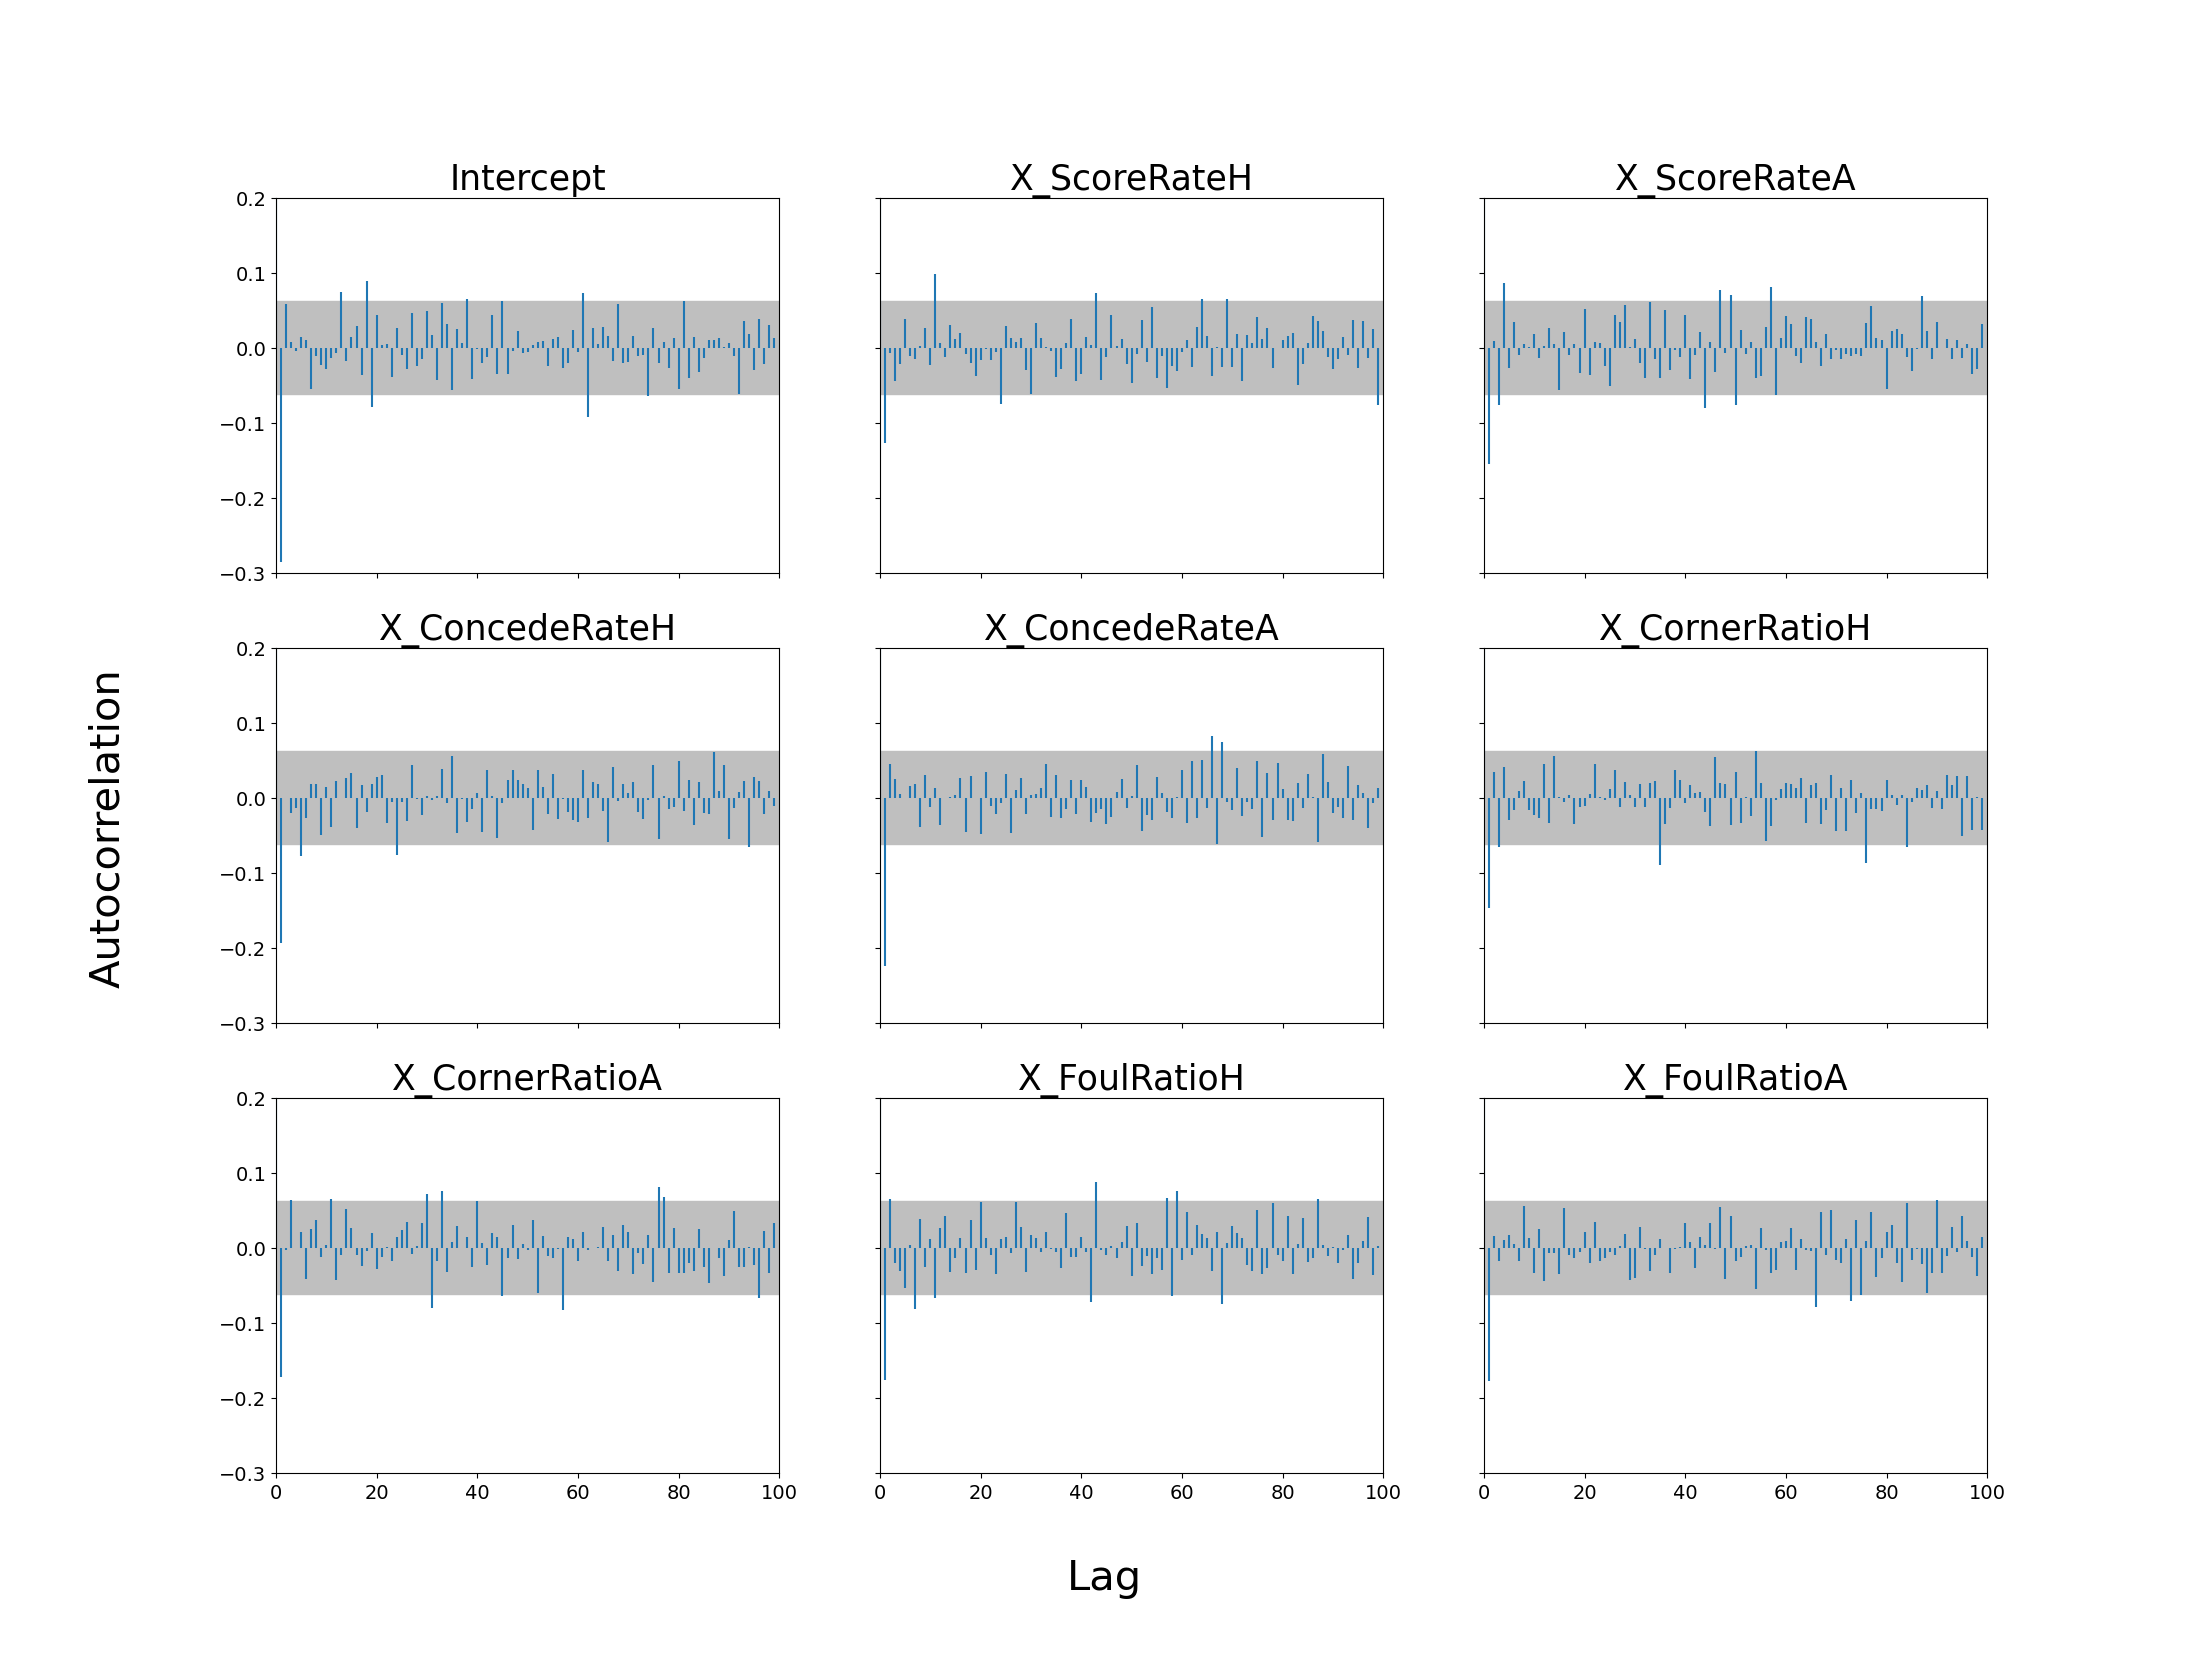
\includegraphics[width=1\columnwidth]{figures/autocorr.png}
\caption{Autocorrelation plots for one chain}
\label{fig:autocorr}
\end{figure}

In Table~\ref{tab:ess_rhat}, we report the ESS and R-hat statistics 
for all regression coefficients. The ESS values are consistently high, 
suggesting efficient sampling. In fact, for some coefficients, the 
ESS exceeds the total number of samples due to the presence of 
negative autocorrelation, which can reduce variance in the sample mean. 
Additionally, all R-hat values are equal to 1.00, indicating that the
 between-chain and within-chain variances are nearly identical, 
 confirming good convergence of the Markov chains.

\begin{table}[ht]
\centering
\begin{tabular}{l|c|c}
\textbf{Regression coefficients} & \textbf{ESS} & \textbf{R-hat} \\
\hline
Intercept        & 6551 & 1.00 \\
X\_ScoreRateH    & 5878 & 1.00 \\
X\_ScoreRateA    & 6180 & 1.00 \\
X\_ConcedeRateH  & 6050 & 1.00 \\
X\_ConcedeRateA  & 6963 & 1.00 \\
X\_CornerRatioH  & 6529 & 1.00 \\
X\_CornerRatioA  & 6416 & 1.00 \\
X\_FoulRatioH    & 6123 & 1.00 \\
X\_FoulRatioA    & 6782 & 1.00 \\
\end{tabular}
\caption{ESS and R-hat diagnostics for regression coefficients}
\label{tab:ess_rhat}
\end{table}
\vspace{-20pt}

\section{Laplace approximation}
\subsection{Implementation}
To implement the Laplace approximation, we 
first derive the negative log-posterior, its gradient,
 and Hessian with respect to the regression coefficients
  \(\boldsymbol{\beta}\) (See Appendix for derivation).
   Since we used a minimizer, we provide
  the negated versions.

Negative log-posterior: 
\begin{align}
-\log p(\boldsymbol{\beta} \mid \mathbf{X}, \mathbf{y}) 
= - \left( \mathbf{y}^\top \mathbf{X}\boldsymbol{\beta} - \mathbf{1}^\top \exp(\mathbf{X}\boldsymbol{\beta}) - \frac{1}{2\alpha} \boldsymbol{\beta}^\top \boldsymbol{\beta} \right)
\end{align}

\noindent where \(\alpha\) is the prior variance parameter for a Gaussian prior \(\boldsymbol{\beta} \sim \mathcal{N}(\mathbf{0}, \alpha \mathbf{I})\).

\noindent The gradient of the negative log-posterior is
\begin{align}
\nabla_{\boldsymbol{\beta}} \left( -\log p(\boldsymbol{\beta} \mid \mathbf{X}, \mathbf{y}) \right) 
&= - \left( \mathbf{X}^\top \mathbf{y} - \mathbf{X}^\top \exp(\mathbf{X}\boldsymbol{\beta}) - \frac{1}{\alpha} \boldsymbol{\beta} \right)
\end{align}

\noindent The Hessian matrix is given by
\[
\mathbf{H} = \mathbf{X}^\top \operatorname{diag}\left(\exp(\mathbf{X}\boldsymbol{\beta})\right) \mathbf{X} + \frac{1}{\alpha} \mathbf{I}
\]


These expressions are used to find the mode of the posterior
 and approximate it with a Gaussian distribution centered at 
 the mode with covariance \(\mathbf{H}^{-1}\).

\subsection{Comparison with MCMC}
To compare the Laplace approximation with the MCMC results, we plot
 the marginal distributions obtained from the approximation in 
 Figure~\ref{fig:approx}. These densities closely resemble those 
 from the MCMC sampling, demonstrating that the Laplace method 
 captures the posterior distributions well. However, unlike the
  MCMC samples, the approximated distributions are obviously exact Normal
   distributions.

\begin{figure}[h]
\centering
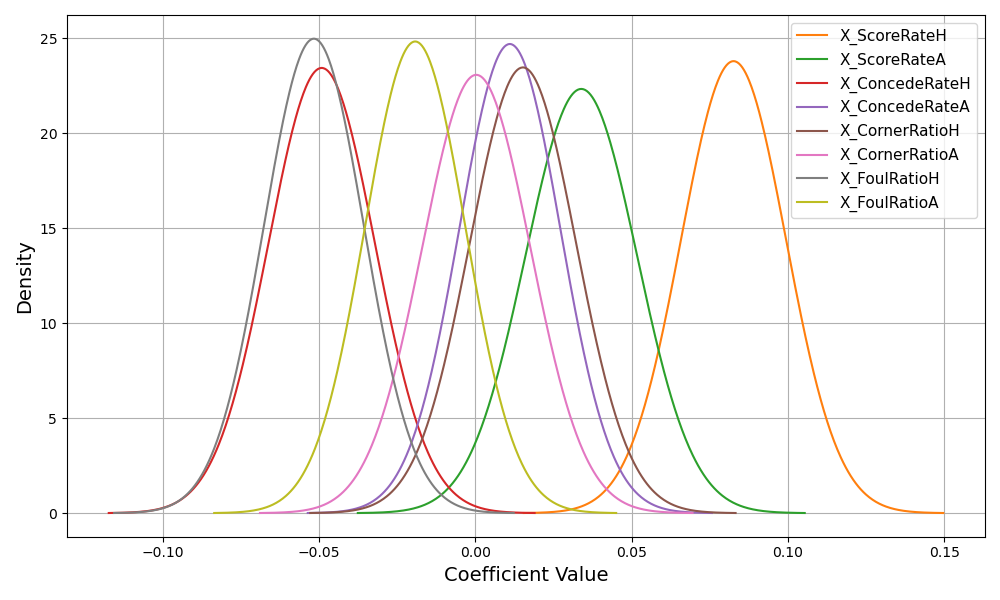
\includegraphics[width=1\columnwidth]{figures/approximation.png}
\caption{Distributions of regression coefficients for the Laplace approximation}
\label{fig:approx}
\end{figure}

\subsection{Predictions for test cases}
Lastly, we use our model to make predictions on the test dataset. 
To obtain the predictive distributions, we first draw 1000 samples from the
 multivariate normal distribution defined by the estimated posterior mean of 
 the regression coefficients and the corresponding covariance matrix (the inverse
  of the Hessian evaluated at the posterior mode of $\boldsymbol{\beta}$). For
   each sampled coefficient vector, we compute the linear predictor, apply the 
   exponential link function of the Poisson GLM to obtain $\lambda-s$, and then draw
    1000 samples from the Poisson distribution for each $\lambda$ to get
     the predictive distribution.

For point predictions, we match the summary statistic of the predictive distribution to the corresponding loss function:
\begin{itemize}
    \item \textbf{Squared error loss:} use the  mean
    \item \textbf{Absolute error loss:} use the median
    \item \textbf{Accuracy:} use the mode 
\end{itemize}

We can see the prediction distributions on Figure~\ref{fig:distr}.

\begin{figure}[h]
\centering
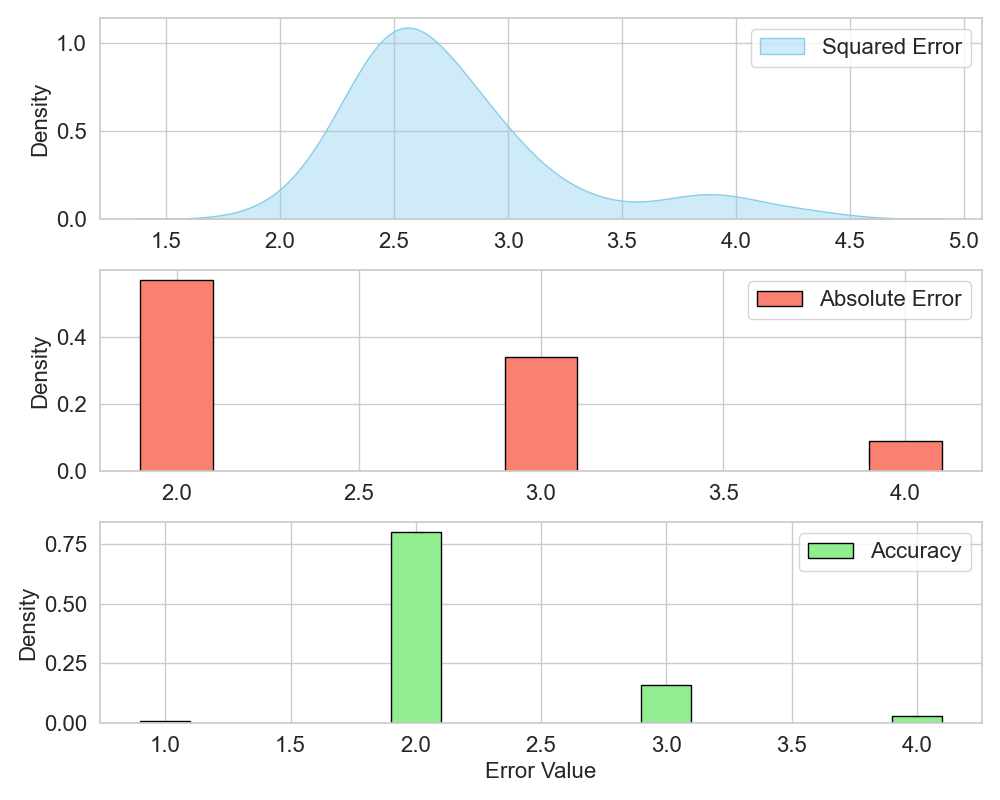
\includegraphics[width=0.9\columnwidth]{figures/distr.png}
\caption{Distributions of predictions for different losses}
\label{fig:distr}
\end{figure}



\newpage
\section{Appendix}
\begin{figure}[h]
\centering
\rotatebox{180}{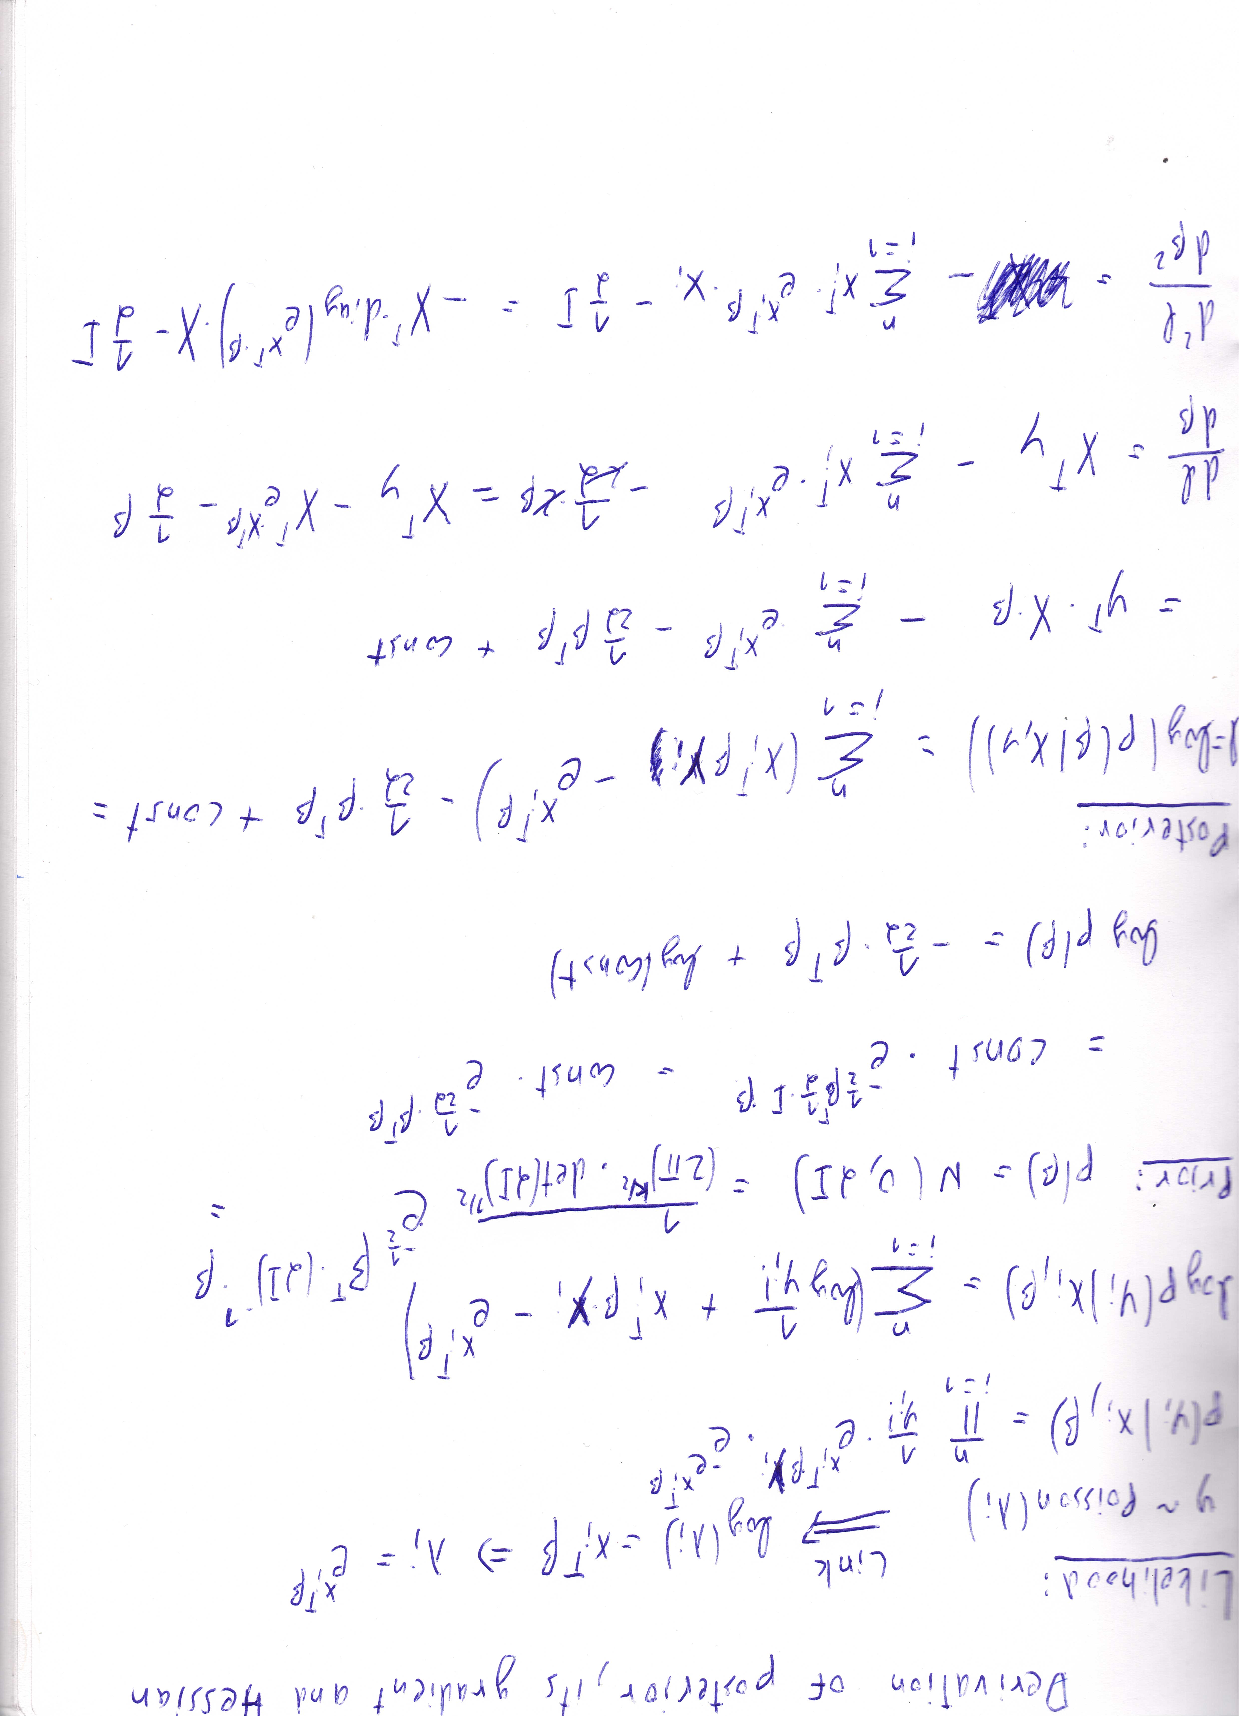
\includegraphics[width=1.75\columnwidth]{figures/derivation.pdf}}
\label{fig:der}
\end{figure}


\bibliographystyle{IEEEtran}
\bibliography{bibliography}

\end{document}
